\chapter{De l'intention au mouvement}\label{ch:g12:brain-and-movement}

Une femme se réveille un matin sans pouvoir bouger son bras ni sa
jambe droits, alors qu'elle les sent, et son genou droit se détend
plus fort que jamais quand le médecin le frappe. L'imagerie montre une
petite zone morte dans la moitié gauche de son cerveau, près du
sommet. Tout ce qui est au-dessous est intact --- les nerfs, la moelle
épinière, les \omterm{def:g12:stretch-reflex:reflex}{arcs réflexes} du chapitre précédent, les muscles --- et
pourtant l'intention de bouger ne les atteint pas. Six mois de
rééducation plus tard, elle marche, et l'imagerie de son cerveau en
activité montre des régions qui s'allument alors qu'elles ne
commandaient pas sa jambe auparavant. Ce chapitre suit un mouvement
volontaire du cortex jusqu'au motoneurone, et montre comment la carte
qui le commande est tracée, croisée, et retracée.

\section{Le cortex moteur}

\begin{definition}[Cortex moteur]\label{def:g12:brain-and-movement:cortex}
Le \emph{cortex moteur primaire}\index{cortex moteur} est une bande du
cortex cérébral qui court sur le sommet de chaque hémisphère, juste en
avant du sillon qui sépare le lobe frontal du lobe pariétal. Ses
\omterm{def:g12:stretch-reflex:neuron}{neurones} sont à l'origine du mouvement volontaire~: leurs axones
descendent par le tronc cérébral et la moelle épinière jusqu'aux
motoneurones des muscles. Cette bande est une \emph{carte} du corps~:
chacune de ses parties commande une partie du corps, dans un ordre qui
va du pied, au sommet de l'hémisphère, au visage, sur son côté, et
l'aire de chaque partie est proportionnelle non à la taille de la
partie du corps mais à la finesse de ses mouvements --- la main et le
visage en occupent l'essentiel.
\end{definition}

\begin{proposition}[La carte est réelle, et croisée]\label{prop:g12:brain-and-movement:map}
Stimuler électriquement un point du \omterm{def:g12:brain-and-movement:cortex}{cortex moteur} produit un mouvement
de la partie du corps correspondante du côté \emph{opposé} du corps~;
l'atteinte d'un point abolit le mouvement volontaire de cette partie
du côté opposé.
\end{proposition}
\begin{proof}[Preuves]
Au cours d'opérations du cerveau sous anesthésie locale, Penfield
(années 1930) a appliqué un courant faible à des points du cortex
exposé et a noté quels muscles bougeaient~: ces points formaient la
carte, avec les aires de la main et du visage hors de proportion avec
leur taille, et chaque mouvement du côté opposé à l'hémisphère
stimulé. L'imagerie fonctionnelle de volontaires en bonne santé qui
bougent un doigt montre une tache d'activité à l'endroit prévu dans
l'hémisphère opposé~; en bougeant le pied, une tache au sommet. Les
accidents vasculaires cérébraux qui détruisent une partie d'un \omterm{def:g12:brain-and-movement:cortex}{cortex
moteur} paralysent les parties cartographiées de l'autre côté, la
sensibilité restant intacte.
\end{proof}

\begin{omfigure}
\begin{tikzpicture}
  \node[anchor=south west, inner sep=0] (img) at (0,0)
    {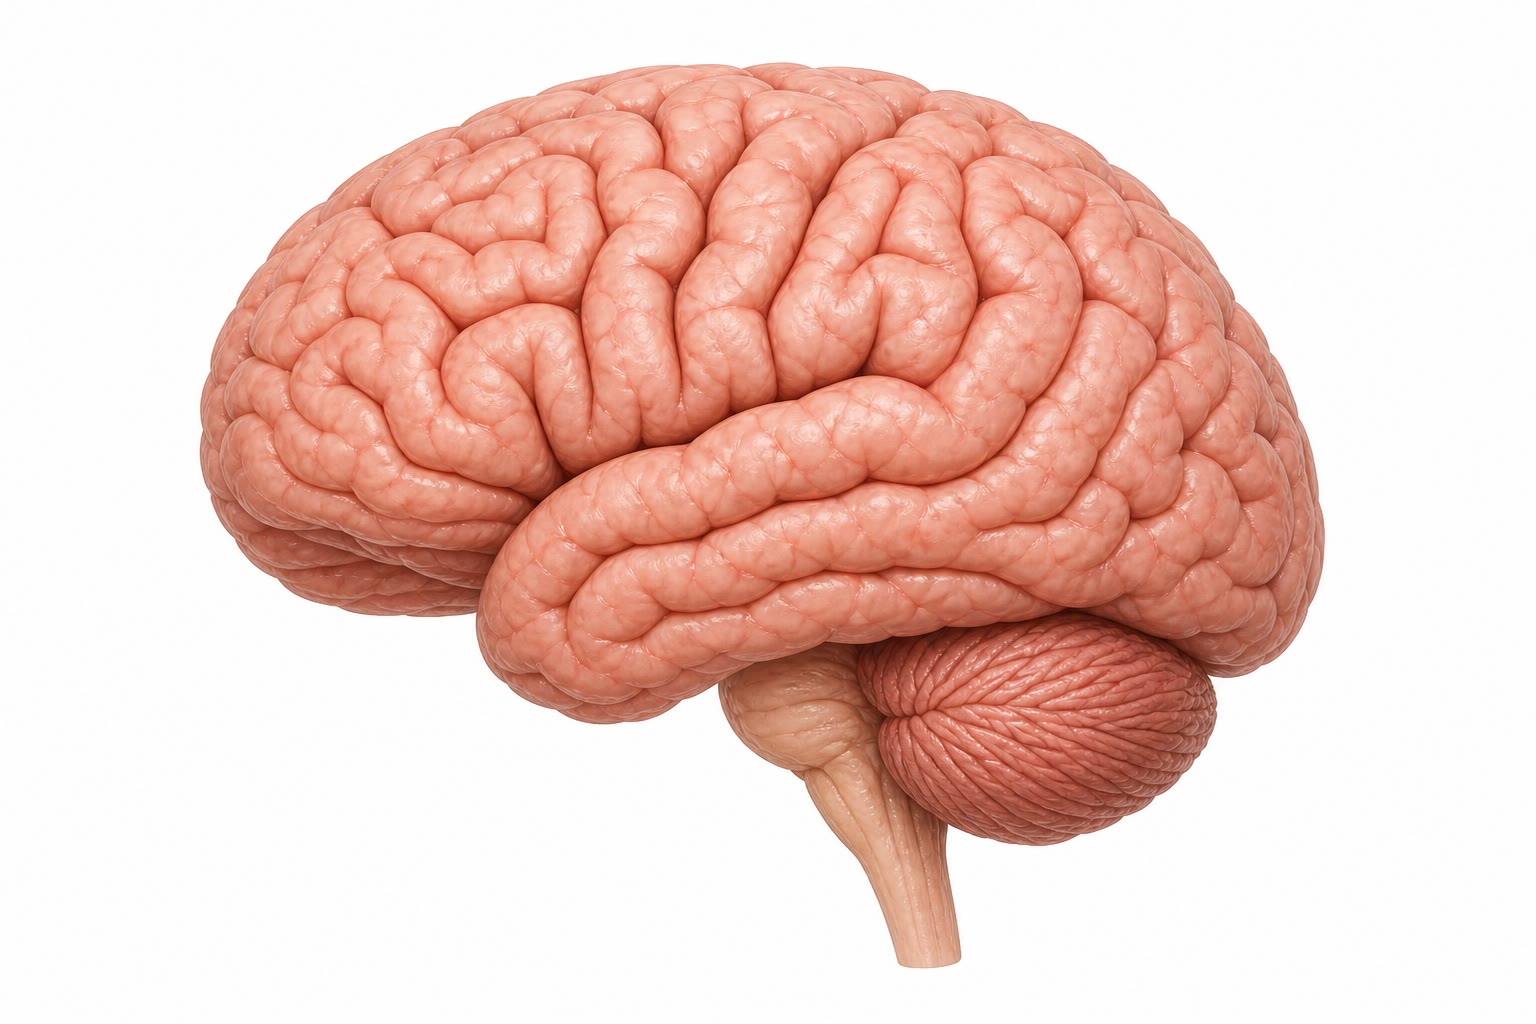
\includegraphics[width=0.52\linewidth]{images/book2/ai/fig-brain-side.jpg}};
  \begin{scope}[x={(img.south east)}, y={(img.north west)},
      every node/.style={font=\small}]
    \draw[omThm, very thick] (0.50,0.90) .. controls (0.53,0.75) .. (0.58,0.55);
    \draw[omDef, thick] (0.52,0.82) -- (0.45,1.08) node[above, align=center] {cortex moteur primaire\\ (bande en avant du sillon central)};
    \draw[omDef, thick] (0.28,0.72) -- (0.10,1.02) node[above] {lobe frontal~: la planification};
    \draw[omDef, thick] (0.72,0.72) -- (0.85,1.02) node[above] {lobe pariétal~: la sensibilité};
    \draw[omDef, thick] (0.70,0.28) -- (1.04,0.20) node[right] {cervelet};
    \draw[omDef, thick] (0.60,0.10) -- (0.60,-0.06) node[below] {tronc cérébral~: le trajet y croise};
  \end{scope}
\end{tikzpicture}

{\small Le cerveau vu de la gauche, avec le \omterm{def:g12:brain-and-movement:cortex}{cortex moteur primaire}
marqué en rouge~: une bande au sommet de l'hémisphère, qui commande le
côté droit du corps. Ses fibres descendantes croisent vers l'autre
côté dans le tronc cérébral.}
\end{omfigure}

\begin{omfigure}
\begin{tikzpicture}
\begin{axis}[
  xbar, bar width=9pt,
  width=0.8\linewidth, height=6cm,
  axis x line=bottom, axis y line=left,
  xmin=0, xmax=35, xlabel={part du cortex moteur (\%)},
  xlabel style={font=\small, at={(axis description cs:0.5,-0.1)}, anchor=north},
  symbolic y coords={orteils et pied, jambe, tronc, bras, main et doigts, visage et langue},
  ytick=data, tick label style={font=\small},
  enlarge y limits=0.12, xtick={0,10,20,30},
  nodes near coords, nodes near coords style={font=\scriptsize, anchor=west},
]
\addplot[fill=omThm!50, draw=omThm] coordinates
  {(4,orteils et pied) (8,jambe) (6,tronc) (14,bras) (32,main et doigts) (30,visage et langue)};
\end{axis}
\end{tikzpicture}

{\small Part approximative du \omterm{def:g12:brain-and-movement:cortex}{cortex moteur} consacrée à chaque partie
du corps. La main et le visage, qui font les mouvements les plus fins,
en prennent près des deux tiers~; le tronc, qui en fait peu, en prend
un vingtième. L'aire suit la précision, non la taille.}
\end{omfigure}

\begin{omfigure}
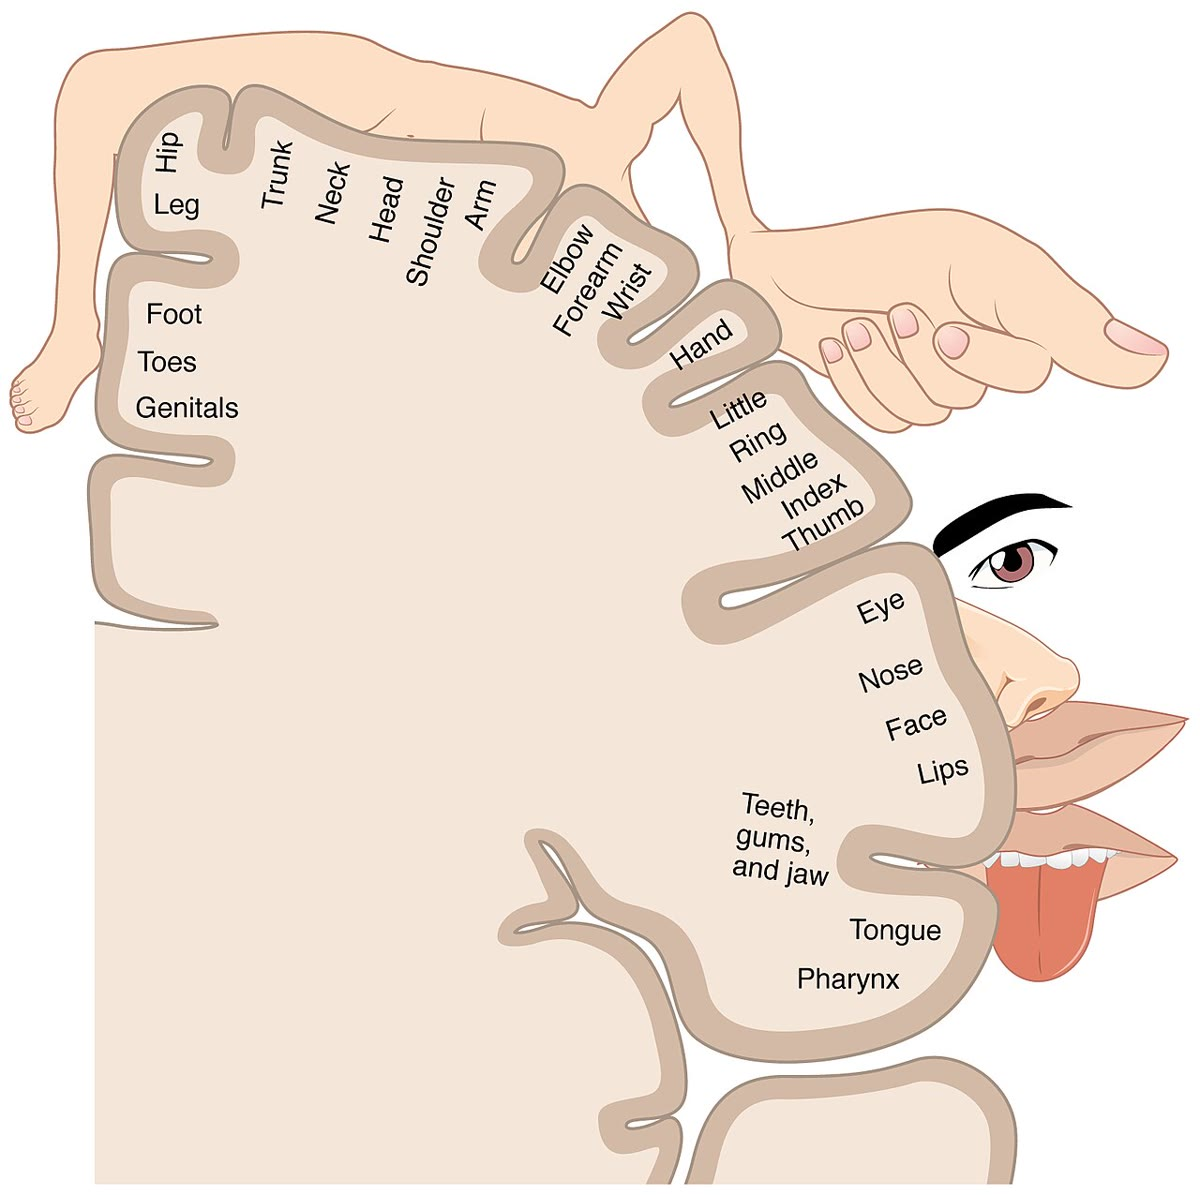
\includegraphics[width=0.5\linewidth]{images/book2/homunculus.jpg}

{\small La carte dessinée sous forme de corps~: chaque partie est dimensionnée par le cortex qu'elle occupe, et posée sur une coupe de l'hémisphère. C'est ici la bande sensitive, juste en arrière de la bande motrice~; la carte motrice a le même ordre et presque les mêmes proportions --- main et visage énormes, tronc et jambe petits. Illustration tirée d'OpenStax \emph{Anatomy and Physiology}, CC~BY~3.0.}
\end{omfigure}

\section{Le trajet descendant}

\begin{proposition}[Du cortex au motoneurone]\label{prop:g12:brain-and-movement:pathway}
Les axones des \omterm{def:g12:stretch-reflex:neuron}{neurones} du \omterm{def:g12:brain-and-movement:cortex}{cortex moteur} forment le \emph{faisceau
corticospinal}\index{faisceau corticospinal}. Il descend par le tronc
cérébral, où la plupart de ses fibres croisent vers l'autre
côté --- ce qui explique que chaque hémisphère commande la moitié
opposée du corps --- et se poursuit dans la moelle épinière, où à
chaque niveau des fibres le quittent pour se terminer sur les
motoneurones des muscles de ce niveau, ou sur des interneurones
voisins. Le motoneurone du \cref{ch:g12:stretch-reflex} est donc le
point de rencontre de deux commandes~: celle de l'\omterm{def:g12:stretch-reflex:reflex}{arc réflexe}, venue
du fuseau neuromusculaire, et celle du cortex, venue d'un mètre plus
haut.
\end{proposition}
\begin{proof}[Preuves]
Suivre les fibres du cortex à travers le tronc cérébral montre le
croisement~; une lésion du faisceau au-dessus du croisement paralyse
le côté opposé, au-dessous, le même côté. Une lésion de la moelle
épinière paralyse tout ce qui est au-dessous de son niveau, des deux
côtés, en épargnant le visage, dont les fibres quittent le faisceau
plus haut~; les \omterm{def:g12:stretch-reflex:reflex}{réflexes} situés au-dessous de la lésion persistent,
puisque leurs arcs sont intacts, et deviennent exagérés, puisque
l'influence amortissante du cortex ne les atteint plus.
\end{proof}

\begin{omfigure}
\begin{tikzpicture}[font=\small, >=Stealth, line cap=round]
  % left hemisphere box, brainstem, cord, muscles
  \draw[thick, fill=omDef!8, rounded corners=10pt] (-3.4,4.2) rectangle (-0.2,5.8);
  \node at (-1.8,5.0) {cortex moteur gauche};
  \draw[thick, fill=omDef!8, rounded corners=10pt] (0.2,4.2) rectangle (3.4,5.8);
  \node at (1.8,5.0) {cortex moteur droit};
  \draw[thick, fill=gray!15] (-0.8,1.6) rectangle (0.8,3.6);
  \node[font=\scriptsize, anchor=east] at (-0.9,3.3) {tronc cérébral};
  \draw[thick, fill=gray!10] (-0.6,-2.4) rectangle (0.6,1.6);
  \node[font=\scriptsize, rotate=90] at (0,-0.4) {moelle épinière};
  % tracts: left cortex -> crosses -> right side of cord -> right muscles
  \draw[very thick, omThm] (-1.8,4.2) -- (-0.4,3.4) -- (-0.4,2.6) -- (0.35,2.0) -- (0.35,-1.6);
  \draw[very thick, omDef] (1.8,4.2) -- (0.4,3.4) -- (0.4,2.6) -- (-0.35,2.0) -- (-0.35,-1.6);
  \node[font=\scriptsize, anchor=west] at (0.9,2.3) {croisement};
  % motor neurons and muscles
  \fill[omThm] (0.35,-1.6) circle (2.5pt); \draw[very thick, omThm] (0.35,-1.6) -- (2.6,-1.6);
  \draw[thick, fill=omThm!25, rounded corners=5pt] (2.6,-2.0) rectangle (3.8,-1.2); \node[font=\scriptsize] at (3.2,-1.6) {jambe droite};
  \fill[omDef] (-0.35,-1.6) circle (2.5pt); \draw[very thick, omDef] (-0.35,-1.6) -- (-2.6,-1.6);
  \draw[thick, fill=omDef!25, rounded corners=5pt] (-3.8,-2.0) rectangle (-2.6,-1.2); \node[font=\scriptsize] at (-3.2,-1.6) {jambe gauche};
  \node[font=\scriptsize, anchor=west, align=left] at (0.9,0.3) {motoneurone~: point de rencontre\\ de la commande du cortex\\ et de l'arc réflexe};
  \draw[gray, thin] (0.9,-0.2) -- (0.5,-1.45);
  \draw[->, thick, gray] (3.2,-2.4) .. controls (2.0,-3.0) and (0.8,-2.6) .. (0.5,-1.8);
  \node[font=\scriptsize, gray, anchor=north] at (2.2,-2.8) {fuseau de la jambe droite (entrée réflexe)};
\end{tikzpicture}

{\small Le \omterm{prop:g12:brain-and-movement:pathway}{faisceau corticospinal}. Les fibres du \omterm{def:g12:brain-and-movement:cortex}{cortex moteur} gauche
(en rouge) croisent dans le tronc cérébral et descendent du côté droit
de la moelle jusqu'aux motoneurones de la jambe droite~; le cortex
droit (en bleu) commande la gauche. Chaque motoneurone reçoit aussi
l'entrée \omterm{def:g12:stretch-reflex:reflex}{réflexe} de son propre muscle.}
\end{omfigure}

\begin{example}[Lire une paralysie]\label{ex:g12:brain-and-movement:paralysis}
Bras et jambe droits paralysés, le visage aussi, la sensibilité
conservée~: une lésion du \omterm{def:g12:brain-and-movement:cortex}{cortex moteur} de l'hémisphère gauche ou de
ses fibres au-dessus du croisement --- la femme du début. Les deux
jambes paralysées, bras et visage épargnés, \omterm{def:g12:stretch-reflex:reflex}{réflexes} des jambes
exagérés~: la moelle épinière atteinte au niveau du bas du dos. Un
seul bras paralysé et flasque, ses \omterm{def:g12:stretch-reflex:reflex}{réflexes} absents~: le nerf ou les
motoneurones eux-mêmes, au-delà desquels plus rien ne peut émettre. La
carte, le croisement et l'arc localisent l'atteinte avant toute
imagerie.
\end{example}

\section{Le motoneurone décide}

\begin{proposition}[L'intégration au motoneurone]\label{prop:g12:brain-and-movement:integration}
Un motoneurone reçoit des milliers de \omterm{def:g12:stretch-reflex:synapse}{synapses}~: des \omterm{def:g12:stretch-reflex:synapse}{synapses}
excitatrices venues du cortex et des fuseaux, des \omterm{def:g12:stretch-reflex:synapse}{synapses}
inhibitrices venues d'interneurones commandés par les fuseaux de
l'antagoniste, par le cortex et par d'autres centres. Chaque signal
qui arrive déplace un peu la tension du \omterm{def:g12:stretch-reflex:neuron}{neurone}, vers le seuil ou à
l'écart~; ces déplacements \emph{s'additionnent} au fil des
millisecondes et sur la surface de la \omterm{def:g10:cells-common-unit:cell}{cellule}, et le \omterm{def:g12:stretch-reflex:neuron}{neurone} n'émet
que lorsque leur somme franchit le seuil. Le motoneurone n'est donc
pas un relais mais un calculateur~: le muscle se contracte quand la
balance de toutes les commandes qui atteignent ses motoneurones le
dit --- la \emph{voie finale commune}\index{voie finale commune} du
mouvement.
\end{proposition}
\begin{proof}[Preuves]
Un enregistrement à l'intérieur d'un motoneurone montre que chaque
entrée excitatrice produit une petite dépolarisation d'un millivolt
environ, bien au-dessous des \qty{15}{mV} nécessaires~; une salve
d'entrées, ou des entrées venues de plusieurs sources à la fois,
sommées jusqu'au seuil, produisent un \omterm{prop:g12:stretch-reflex:actionpotential}{potentiel d'action}~; une entrée
inhibitrice qui arrive au même instant en annule une excitatrice. La
force d'une contraction volontaire croît avec le nombre de
motoneurones recrutés et avec leur rythme d'émission, et le \omterm{def:g12:stretch-reflex:reflex}{réflexe}
rotulien est plus fort quand le sujet serre le poing --- l'excitation
du cortex s'ajoutant à celle du fuseau.
\end{proof}

\begin{omfigure}
\begin{tikzpicture}
\begin{axis}[
  width=0.9\linewidth, height=5.6cm,
  axis x line=bottom, axis y line=left,
  xmin=0, xmax=40, ymin=-80, ymax=40,
  xlabel={temps (ms)}, ylabel={tension du motoneurone (mV)},
  xlabel style={font=\small, at={(axis description cs:0.5,-0.12)}, anchor=north},
  ylabel style={font=\small},
  tick label style={font=\small}, xtick={0,10,20,30,40}, ytick={-70,-55,0,30},
  clip=false,
]
\addplot[thick, omDef] coordinates {(0,-70) (5,-70) (5.5,-66) (8,-68) (10,-70) (14,-70) (14.5,-66) (16,-64) (17,-61) (18.5,-58) (19.5,-55) (20,-30) (20.5,30) (21,0) (21.5,-50) (22,-75) (25,-72) (28,-70) (30,-70) (30.5,-66) (31.5,-70) (32,-74) (34,-70) (40,-70)};
\draw[dashed, gray] (axis cs:0,-55) -- (axis cs:40,-55);
\node[font=\scriptsize, gray, anchor=south west] at (axis cs:0.3,-55) {seuil};
\node[font=\scriptsize, anchor=south] at (axis cs:9,-67.5) {une entrée excitatrice};
\node[font=\scriptsize, anchor=south, align=center] at (axis cs:11.5,-45) {quatre entrées en succession\\ rapide~: la somme atteint le seuil};
\node[font=\scriptsize, anchor=south, align=center] at (axis cs:31,-58) {excitatrice + inhibitrice~:\\ elles s'annulent};
\end{axis}
\end{tikzpicture}

{\small L'intégration par un motoneurone. Une seule entrée excitatrice
le dépolarise de quelques millivolts puis s'estompe~; plusieurs,
arrivant en quelques millisecondes, s'additionnent jusqu'au seuil et
le \omterm{def:g12:stretch-reflex:neuron}{neurone} émet~; une entrée inhibitrice arrivant avec une excitatrice
l'annule.}
\end{omfigure}

\begin{example}[Tenir un verre]\label{ex:g12:brain-and-movement:glass}
En soulevant un verre plein, le cortex envoie une excitation soutenue
aux motoneurones du bras~; les fuseaux, étirés à mesure que le verre
penche, ajoutent la leur~; les interneurones des antagonistes
soustraient quand le mouvement dépasse la cible~; le cervelet,
comparant le mouvement voulu et le mouvement réel, corrige la commande
du cortex quelques dizaines de millisecondes plus tard. Chaque
motoneurone fait la somme de toute cette conversation et émet juste ce
qu'il faut. La souplesse du mouvement est l'équilibre de ces sommes.
\end{example}

\section{Une carte que l'on peut retracer}

\begin{proposition}[La plasticité du cortex moteur]\label{prop:g12:brain-and-movement:plasticity}
La carte motrice n'est pas figée. Répéter un mouvement agrandit l'aire
corticale qui le commande et affine ses connexions~; l'aire d'un
membre rétrécit quand le membre est immobilisé et, après une
amputation, elle est reprise par les parties voisines. Après un
accident vasculaire cérébral, le cortex intact autour de la lésion, et
l'aire correspondante de l'autre hémisphère, peuvent apprendre à
commander les muscles atteints --- à condition qu'on s'en serve~: la
rééducation agit en forçant le mouvement, de façon répétée, pour que
les circuits survivants soient sélectionnés et renforcés. La
plasticité du \cref{ch:g11:vision-and-brain} vaut pour le côté du
cerveau qui commande comme pour celui qui perçoit.
\end{proposition}
\begin{proof}[Preuves]
L'imagerie du cortex de violonistes montre une aire agrandie pour les
doigts de la main gauche, en proportion de l'âge auquel ils ont
commencé~; après cinq jours d'\omterm{def:g10:sport-and-health:training}{entraînement} à une séquence de doigts,
des volontaires ordinaires montrent une aire mesurablement agrandie
pour ces doigts, qui rétrécit de nouveau si l'\omterm{def:g10:sport-and-health:training}{entraînement} cesse.
Après un accident vasculaire cérébral, les patients dont le bras
paralysé est entraîné intensivement --- le bon bras étant
immobilisé --- récupèrent plus de fonction que ceux qui compensent
avec le bon bras, et l'imagerie montre que le mouvement retrouvé est
commandé par des régions voisines de la lésion. Des singes dont l'aire
des doigts est lésée ne retrouvent le mouvement des doigts que si l'on
fait travailler ces doigts.
\end{proof}

\begin{omfigure}
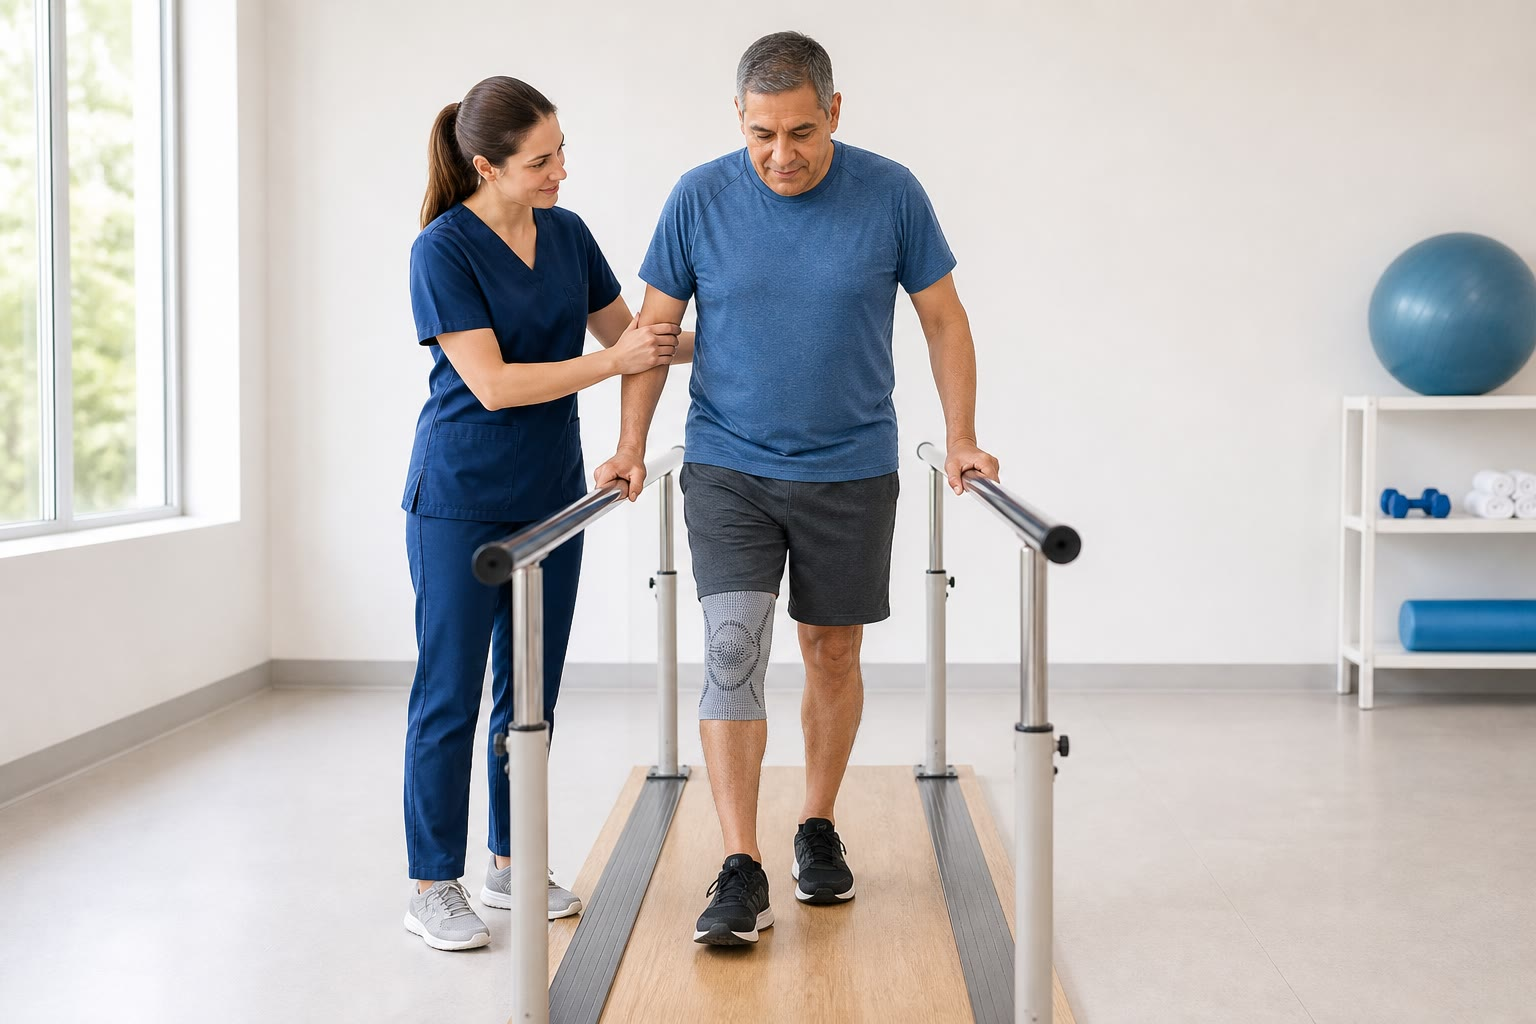
\includegraphics[width=0.56\linewidth]{images/book2/ai/g12-move-rehab.jpg}

{\small La rééducation après un accident vasculaire cérébral~:
réapprendre à marcher entre des barres parallèles. Chaque pas forcé
sélectionne et renforce les circuits survivants capables de commander
la jambe, et la carte corticale est retracée autour de la lésion.}
\end{omfigure}

\begin{example}[Six mois après l'accident]\label{ex:g12:brain-and-movement:sixmonths}
Semaine 1~: la jambe droite ne bouge pas~; ses \omterm{def:g12:stretch-reflex:reflex}{réflexes} sont exagérés.
Semaines 2 à 6~: le kinésithérapeute mobilise la jambe, puis fait
tenter à la patiente chaque mouvement~; une contraction faible
revient. Mois 2 à 4~: marche entre les barres, mille pas par jour~;
l'imagerie montre l'activité qui s'étend dans le cortex autour de la
lésion et dans l'autre hémisphère. Mois 6~: marche avec une canne. La
lésion n'a pas guéri --- les \omterm{def:g12:stretch-reflex:neuron}{neurones} du cortex ne repoussent
pas --- mais des circuits voisins ont été recrutés, et chaque étape de
la récupération s'est faite en tentant le mouvement.
\end{example}

\begin{method}[Localiser un trouble moteur]\label{met:g12:brain-and-movement:locate}
\begin{enumerate}
  \item Quelles parties sont atteintes~? Un côté du corps, visage
        compris~: l'hémisphère opposé ou ses fibres au-dessus du
        croisement. Les deux côtés au-dessous d'un niveau, visage
        épargné~: la moelle épinière à ce niveau. Un seul membre ou un
        seul groupe de muscles~: son nerf ou ses motoneurones.
  \item Les \omterm{def:g12:stretch-reflex:reflex}{réflexes} sont-ils conservés~? Exagérés~: l'arc est intact
        et l'amortissement cortical est perdu (une lésion au-dessus du
        motoneurone). Absents~: l'arc lui-même est rompu (le
        motoneurone, le nerf ou le muscle).
  \item La sensibilité est-elle conservée~? Un déficit purement moteur
        désigne le trajet moteur~; un déficit mixte, une lésion qui
        touche les deux.
  \item Que peut-on récupérer~? Les lésions corticales, par la
        plasticité et l'\omterm{def:g10:sport-and-health:training}{entraînement}~; une moelle ou un nerf
        sectionnés, bien moins~; les maladies du muscle et du
        motoneurone, selon leur cause.
\end{enumerate}
\end{method}

\begin{remark}[La dernière boucle de l'année]\label{rem:g12:brain-and-movement:loop}
L'intention de bouger est un motif de \omterm{prop:g12:stretch-reflex:actionpotential}{potentiels d'action} dans une
bande de cortex~; elle descend un mètre d'axone, croise, et est pesée
par un motoneurone face au \omterm{def:g12:stretch-reflex:reflex}{réflexe} du muscle qu'elle va mouvoir~; le
muscle se contracte par le glissement des filaments, payé par l'\omterm{def:g12:respiration-fermentation:atp}{ATP}
des \omterm{def:g10:cells-common-unit:organelle}{mitochondries}, à partir du glucose que le foie a libéré sous l'œil
du pancréas et de l'oxygène que le cœur et les poumons ont
délivré --- et le cortex qui a donné l'ordre a été façonné, par son
propre usage, en la carte qu'il est. Chaque chapitre de ce livre a été
un morceau de cette boucle. Les volumes qui suivent ouvrent chaque
morceau davantage~; aucun ne change la boucle.
\end{remark}

\section{Exercices}

\begin{exercise}[$\star$]\label{exo:g12:brain-and-movement:1}
Où se trouve le \omterm{def:g12:brain-and-movement:cortex}{cortex moteur primaire}, et que représente sa carte~?
\end{exercise}

\begin{exercise}[$\star$]\label{exo:g12:brain-and-movement:2}
Décrire le \omterm{prop:g12:brain-and-movement:pathway}{faisceau corticospinal}, du cortex à un muscle de la jambe,
en nommant l'endroit où il croise.
\end{exercise}

\begin{exercise}[$\star$]\label{exo:g12:brain-and-movement:3}
Pourquoi la main occupe-t-elle plus de \omterm{def:g12:brain-and-movement:cortex}{cortex moteur} que tout le
tronc~?
\end{exercise}

\begin{exercise}[$\star$]\label{exo:g12:brain-and-movement:4}
Que signifie «~\omterm{prop:g12:brain-and-movement:integration}{voie finale commune}~» pour le motoneurone~?
\end{exercise}

\begin{exercise}[$\star$]\label{exo:g12:brain-and-movement:5}
Donner deux preuves que la carte motrice peut changer.
\end{exercise}

\begin{exercise}[$\star\star$]\label{exo:g12:brain-and-movement:6}
D'après la figure de l'intégration, de combien une seule entrée
excitatrice dépolarise-t-elle le \omterm{def:g12:stretch-reflex:neuron}{neurone}, combien en faut-il en
quelques millisecondes pour atteindre le seuil, et que se passe-t-il
quand une entrée inhibitrice coïncide avec une entrée excitatrice~?
\end{exercise}

\begin{exercise}[$\star\star$]\label{exo:g12:brain-and-movement:7}
Un patient ne peut bouger ni le côté gauche du visage ni le bras
gauche~; la jambe gauche est faible. Localiser la lésion, à l'aide de
la carte et du croisement.
\end{exercise}

\begin{exercise}[$\star\star$]\label{exo:g12:brain-and-movement:8}
Expliquer pourquoi le \omterm{def:g12:stretch-reflex:reflex}{réflexe} rotulien est exagéré après un accident
vasculaire cérébral qui paralyse la jambe, et aboli quand le nerf de
la jambe est sectionné.
\end{exercise}

\begin{exercise}[$\star\star$]\label{exo:g12:brain-and-movement:9}
Chez une personne dont la moelle épinière est sectionnée au milieu du
dos~: quels mouvements sont perdus, quels \omterm{def:g12:stretch-reflex:reflex}{réflexes} subsistent, et
pourquoi le visage n'est-il pas atteint~?
\end{exercise}

\begin{exercise}[$\star\star$]\label{exo:g12:brain-and-movement:10}
Expliquer, par l'intégration, pourquoi serrer les poings rend le
\omterm{def:g12:stretch-reflex:reflex}{réflexe} rotulien plus fort.
\end{exercise}

\begin{exercise}[$\star\star$]\label{exo:g12:brain-and-movement:11}
L'aire des doigts d'une pianiste est plus grande que celle d'une
non-musicienne, et plus grande encore si elle a commencé avant l'âge
de sept ans. Interpréter ces deux faits.
\end{exercise}

\begin{exercise}[$\star\star\star$]\label{exo:g12:brain-and-movement:12}
Après un accident vasculaire cérébral, immobiliser le bon bras et
forcer l'usage du bras paralysé donne une meilleure récupération que
de laisser le patient compenser. Expliquer par la sélection des
circuits, et rapprocher ce fait des chatons du
\cref{ch:g11:vision-and-brain}.
\end{exercise}

\begin{exercise}[$\star\star\star$]\label{exo:g12:brain-and-movement:13}
Un amputé sent sa main absente quand on lui touche la joue, et
l'imagerie montre que l'aire du visage s'est étendue dans l'ancienne
aire de la main. Expliquer, et dire ce que cela laisse prévoir pour le
\omterm{def:g12:brain-and-movement:cortex}{cortex moteur} du même côté.
\end{exercise}

\begin{exercise}[$\star\star\star$]\label{exo:g12:brain-and-movement:14}
Une maladie détruit les motoneurones de la moelle épinière alors que
le cortex est intact~; une autre détruit le \omterm{def:g12:brain-and-movement:cortex}{cortex moteur} alors que
les motoneurones sont intacts. Comparer les deux patients~: paralysie,
\omterm{def:g12:stretch-reflex:reflex}{réflexes}, fonte musculaire, et ce qu'une interface cerveau--machine
pourrait faire pour chacun.
\end{exercise}

\begin{exercise}[$\star\star\star$]\label{exo:g12:brain-and-movement:15}
«~Apprendre un mouvement, c'est changer les muscles.~» Corriger cette
phrase en un paragraphe, à l'aide de la carte corticale, de
l'intégration au motoneurone, et de la plasticité.
\end{exercise}

\section{Problème~: l'hémisphère gauche}

\begin{problem}[{Problème du week-end --- un accident vasculaire
cérébral lu des symptômes jusqu'à la lésion, l'arithmétique du
motoneurone, la carte retracée en six mois, et toute la boucle de
l'année refermée}]
\label{pb:g12:brain-and-movement:1}
Une femme de 62 ans se réveille avec le bras et la jambe droits
paralysés et le côté droit du visage tombant~; la sensibilité est
normale~; le \omterm{def:g12:stretch-reflex:reflex}{réflexe} rotulien droit est exagéré, le gauche normal.
L'imagerie montre une lésion de \qty{2}{cm} dans la partie supérieure
de l'hémisphère gauche.

\medskip
\noindent\textbf{Partie I --- Localiser.}
\begin{enumerate}
  \item Expliquer pourquoi la lésion est à gauche alors que le déficit
        est à droite.
  \item Quelle partie de la carte est atteinte~? Justifier à partir
        des trois parties du corps concernées.
  \item Pourquoi la sensibilité est-elle normale~? Quelle bande de
        cortex est épargnée~?
  \item Pourquoi le \omterm{def:g12:stretch-reflex:reflex}{réflexe} rotulien droit est-il exagéré plutôt
        qu'aboli~?
  \item Un second patient a la même paralysie mais avec le \omterm{def:g12:stretch-reflex:reflex}{réflexe}
        rotulien absent et des muscles qui fondent. Localiser sa
        lésion et expliquer la différence.
\end{enumerate}

\medskip
\noindent\textbf{Partie II --- L'arithmétique du motoneurone.}
Un motoneurone de la jambe droite a un seuil situé \qty{15}{mV}
au-dessus de sa tension de repos. Chaque entrée corticale le
dépolarise de \qty{1}{mV}, chaque entrée du fuseau de \qty{2}{mV},
chaque entrée inhibitrice venue de l'interneurone de l'antagoniste de
\qty{-2}{mV}~; les entrées s'additionnent si elles arrivent en moins
de \qty{5}{ms}.
\begin{enumerate}[resume]
  \item Avant l'accident, un pas volontaire envoyait 12 entrées
        corticales et le fuseau 3, en \qty{5}{ms}. Le \omterm{def:g12:stretch-reflex:neuron}{neurone}
        émettait-il~?
  \item Pendant le même pas, 2 entrées inhibitrices arrivaient aussi.
        Refaire la somme.
  \item Après l'accident, les entrées corticales sont nulles. Quelle
        est la somme lors d'une tentative de pas~? Que fait la jambe~?
  \item Le médecin frappe le genou~: le fuseau envoie 10 entrées en
        \qty{5}{ms}. Avant l'accident, le cortex envoyait aussi 3
        entrées inhibitrices (d'amortissement) pendant un coup~;
        après, aucune. Calculer les sommes et expliquer le \omterm{def:g12:stretch-reflex:reflex}{réflexe}
        exagéré.
  \item Trois mois plus tard, les entrées corticales sont remontées à
        8 par pas. Avec les 3 du fuseau, le \omterm{def:g12:stretch-reflex:neuron}{neurone} émet-il~? À quoi
        vous attendez-vous que le mouvement ressemble~?
\end{enumerate}

\medskip
\noindent\textbf{Partie III --- La carte retracée.}
\begin{enumerate}[resume]
  \item Les \omterm{def:g12:stretch-reflex:neuron}{neurones} morts de la lésion ne repoussent pas. D'où
        peuvent venir les entrées corticales de la question 10~?
  \item La rééducation exige que la patiente tente le mouvement des
        milliers de fois. Expliquer, par la plasticité, pourquoi le
        fait de tenter compte, et pourquoi il ne suffit pas que le
        kinésithérapeute mobilise passivement la jambe.
  \item L'imagerie du quatrième mois montre une activité dans l'aire
        de la jambe de l'hémisphère droit pendant un pas de la jambe
        droite. Quelles fibres pourraient porter cette commande,
        compte tenu du croisement~?
  \item La main droite de la patiente récupère moins que sa jambe.
        Proposer une explication à partir de la carte et des exigences
        des mouvements de la main.
  \item Comparer sa récupération avec celle d'un chaton dont l'\omterm{def:g11:the-eye:parts}{œil}
        fermé est rouvert après la période critique. Qu'y a-t-il de
        semblable, qu'y a-t-il de différent~?
\end{enumerate}

\medskip
\noindent\textbf{Partie IV --- La boucle refermée.}
\begin{enumerate}[resume]
  \item Suivre un pas de sa marche retrouvée, du cortex à la
        contraction~: nommer le faisceau, le croisement, le point de
        rencontre, le transmetteur au muscle, la source de l'\omterm{def:g12:respiration-fermentation:atp}{ATP} du
        muscle.
  \item Ce pas coûte à ses muscles de l'\omterm{def:g12:respiration-fermentation:atp}{ATP} fabriqué à partir du
        glucose libéré par le foie. Nommer l'\omterm{def:g11:hormones-and-reproduction:hormone}{hormone} qui a permis au
        foie de le libérer et l'organe qui a mesuré le besoin.
  \item L'oxygène de cet \omterm{def:g12:respiration-fermentation:atp}{ATP} a été délivré par un cœur qui battait
        plus vite. Nommer les deux mécanismes qui en ont élevé le
        rythme au début de la marche.
  \item Sa récupération a dépendu de la plasticité~; son accident,
        d'une artère bouchée~; sa survie, de l'\omterm{def:g12:innate-immunity:immunity}{immunité innée} et
        adaptative face aux infections d'un lit d'hôpital. Nommer un
        chapitre de ce volume pour chacun de ces points.
  \item Énoncer le résultat~: le côté et la bande de cortex où siège
        la lésion, la somme d'entrées qui fait émettre un motoneurone,
        et la propriété du cortex qui lui a rendu sa jambe.
\end{enumerate}
\end{problem}
